%%%%%%%%%%%%%%%%%%%%%%%%%%%%%%%%%%%%%%%%%
% NIWeek 2014 Poster by T. Reveyrand
% www.microwave.fr
% http://www.microwave.fr/LaTeX.html
% ---------------------------------------
% 
% Original template created by:
% Brian Amberg (baposter@brian-amberg.de)
%
% This template has been downloaded from:
% http://www.LaTeXTemplates.com
%
% License:
% CC BY-NC-SA 3.0 (http://creativecommons.org/licenses/by-nc-sa/3.0/)
%
%%%%%%%%%%%%%%%%%%%%%%%%%%%%%%%%%%%%%%%%%

%----------------------------------------------------------------------------------------
%	PACKAGES AND OTHER DOCUMENT CONFIGURATIONS
%----------------------------------------------------------------------------------------

\documentclass[a0paper,portrait]{baposter}

\usepackage[font=small,labelfont=bf]{caption} % Required for specifying captions to tables and figures
\usepackage{booktabs} % Horizontal rules in tables
\usepackage{relsize} % Used for making text smaller in some places

\usepackage{amsmath,amsfonts,amssymb,amsthm} % Math packages
\usepackage{eqparbox}

\usepackage{textcomp}

\graphicspath{{figures/}} % Directory in which figures are stored

 \definecolor{bordercol}{RGB}{40,40,40} % Border color of content boxes
 \definecolor{headercol1}{RGB}{186,215,230} % Background color for the header in the content boxes (left side)
 \definecolor{headercol2}{RGB}{120,120,120} % Background color for the header in the content boxes (right side)
 \definecolor{headerfontcol}{RGB}{0,0,0} % Text color for the header text in the content boxes
 \definecolor{boxcolor}{RGB}{210,235,250} % Background color for the content in the content boxes


\begin{document}

\background{ % Set the background to an image (background.pdf)
\begin{tikzpicture}[remember picture,overlay]
\draw (current page.north west)+(-2em,2em) node[anchor=north west]
{
\includegraphics[height=1.1\textheight]{background}};
\end{tikzpicture}
}

\begin{poster}{
grid=false,
borderColor=bordercol, % Border color of content boxes
headerColorOne=headercol1, % Background color for the header in the content boxes (left side)
headerColorTwo=headercol2, % Background color for the header in the content boxes (right side)
headerFontColor=headerfontcol, % Text color for the header text in the content boxes
boxColorOne=boxcolor, % Background color for the content in the content boxes
headershape=roundedright, % Specify the rounded corner in the content box headers
headerfont=\Large\sf\bf, % Font modifiers for the text in the content box headers
textborder=rectangle,
background=user,
headerborder=open, % Change to closed for a line under the content box headers
boxshade=plain
}
{
\includegraphics[scale=0.2]{ustcblue.jpg}}
%
%----------------------------------------------------------------------------------------
%	TITLE AND AUTHOR NAME
%----------------------------------------------------------------------------------------
%
{ \bf  \huge {Status of design and development of CEPC-DHCAL readout electronics} } % Poster title
{\vspace{0.3em} \smaller Yu Wang$^{1,2}$, Daojin Hong$^1$, Jianbei Liu$^1$, Shubin Liu$^{1,2}$, Changqing Feng\'c$^{1,2}$, Yi Zhou$^1$   \\  % Author names
  
\smaller $^1$\it {University of Science and Technology of China} \\ $^2$\it{State Key Laboratory of Particle Detection and Electronics} } % Author email addresses
{
\includegraphics[scale=0.45]{NI.jpg}} % University/lab logo

%----------------------------------------------------------------------------------------
%	INTRODUCTION
%----------------------------------------------------------------------------------------
\headerbox{Introduction}{name=introduction,column=0,row=0, span=3}{
\begin{itemize} 
	\item The goal of this research is to provide a feasible readout scheme for CEPC DHCAl. As the active detector element of sampling calorimeter has finely segmented readout pads of $1\times1cm^2$, it's a real challenge to access huge mount data from calorimeter.
	\vspace{-0.2cm}
	\item In PFA-based calorimeters, simulation results suggest that for readout segments as small as $1cm^2$, simple hit counting is already a good energy measurement for hadrons, so called DHCAL. A more general calorimeter with multi-threshold readout (e.g. 3 thresholds) records more detailed hit information and has better energy for jet energy above 40GeV, a so-called Semi-Digital Hadron Calorimeter (SDHCAL)
	\vspace{-0.1cm}
	\item In out research, a double layer GEM using self-stretching technique has been used. It consists of 3mm drift gap, 1mm transfer gap and 1mm induction gap and the effective area is $30\times30cm^2$with the readout pads small as $1\times1cm^2$.
	\item The chip choosen to readout is a tri-threshold ASIC called MICROROC (MICRO-mesh gaseous structure Read-Out Chip)
\end{itemize}
}


%----------------------------------------------------------------------------------------
%	CALIBRATION
%----------------------------------------------------------------------------------------

\headerbox{MICROROC}{name=Microroc,column=0,span=1,below=introduction}{
MICROROC is a 64-channel Semi-Digital readout chip.\\ Each channel of the MICROROC chip has:
\begin{itemize}
	\item A very low noise fixed gain charge preamplifier, able to handle a dynamic range from 1 fC to 500fC
	\item Two different adjustable shaper. A high gain shaper for small signal and a low gain shaper for large signal
	\item Three comparators for tri-threshold readout
	\item a random access memory used as a digital buffer
\end{itemize}
\begin{enumerate}
\item A relative VNA calibration creates an error-term matrix related to ports 1 and 2:
\begin{equation*}
\begin{pmatrix} a_ 1 \\  b_1 \\  a_2 \\ b_2 \end{pmatrix}=K\begin{bmatrix} 1 & \beta_1  & 0 & 0\\  \gamma_1 &  \delta_1  & 0 & 0 \\ 0 & 0 & \alpha_2 & \beta_2 \\ 0 & 0 &  \gamma_2 &  \delta_2 \end{bmatrix}.\begin{pmatrix} r_ 1 \\  r_2 \\  r_3 \\ r_4 \end{pmatrix}
\label{eq:cal_2_ports}
\end{equation*}

\item The power calibration gives $|K|$
\item The phase calibration yields $\arg\{K\}$
\end{enumerate}

Power and phase calibration are performed at an auxiliary reference plane ($P_{aux}$) after its own 1-port SOL coaxial calibration:

\begin{equation*}
\begin{pmatrix} a_{aux} \\  b_{aux} \end{pmatrix}=K_{aux}\begin{bmatrix} 1 & \beta_{aux} \\  \gamma_{aux} &  \delta_{aux} \end{bmatrix}.\begin{pmatrix} r_1 \\  r_2  \end{pmatrix}
\label{eq:cal_port_aux}
\end{equation*}

\begin{center}
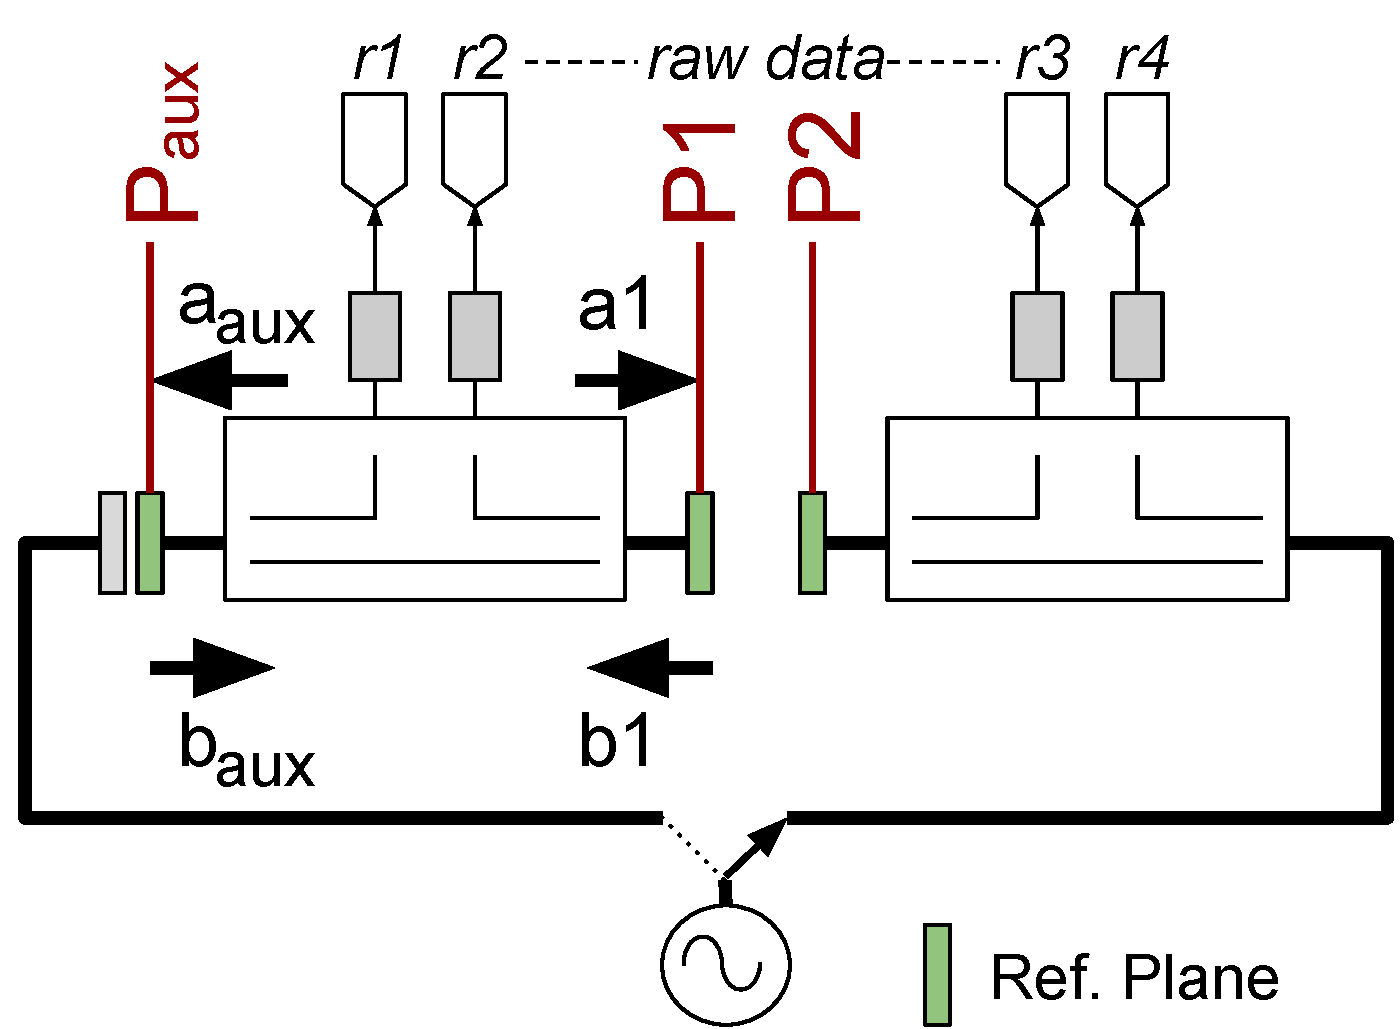
\includegraphics[width=0.7\linewidth]{CALIBRATION.pdf}
\end{center}

\textbf{$\Rightarrow$ Power} calibration at $P_{aux}$ reference plane requires the connection of a power sensor. According to the measured value, in $dBm$, we can calculate $|K_{aux}|$ such as:
\begin{equation*}
|K_{aux}|=\left|{\frac{10^{(Power-10)/20}}{ r_1 + \beta_{aux} . r_2}}\right|
\label{eq:cal_power}
\end{equation*}

\textbf{$\Rightarrow$ Phase} calibration at $P_{aux}$ is performed by connecting a direct receiver (e.g. $r_3$) at $P_{aux}$:
\begin{equation*}
\arg\{K_{aux}\}=\arg\left\{{\frac{r_3}{ r_1 + \beta_{aux} . r_2}}\right\}
\label{eq:cal_phase}
\end{equation*}

\textbf{$\Rightarrow$ Reciprocity} transfers the absolute calibration from $P_{aux}$ to ports 1 and 2 ($P1$ and $P2$):
\begin{equation*}
K=\pm\sqrt{1/Det\{[M]\}}
\label{eq:reciprocity_1}
\end{equation*}
with
\begin{equation*}
M=\begin{bmatrix} 1 & \beta_1  \\  \gamma_1 &  \delta_1 \end{bmatrix}. {\left [ K_{aux}.\begin{bmatrix} 1 & \beta_{aux}  \\  \gamma_{aux} &  \delta_{aux}  \end{bmatrix} \right]}^{-1} 
\label{eq:reciprocity_2}
\end{equation*}
}


%----------------------------------------------------------------------------------------
%	OTHER INSTRUMENTATION
%----------------------------------------------------------------------------------------
\headerbox{Time-domain instrumentation for non-linear devices}{name=instruments,span=2,column=1,row=1, below=introduction}{ % To reduce this block to 1 column width, remove 'span=2'

\begin{center}
\resizebox{0.9\textwidth}{!}{\begin{minipage}{\textwidth}
\begin{tabular}{l l l l}
\toprule
\textbf{Name} & \textbf{Manufacturer} & \textbf{Receivers} & \textbf{Availability}\\
\midrule
MTA (requires two synchronized) & HP & Sampler & Discontinued \\
LSNA & Agilent & Sampler & Discontinued \\
PNA-X + Nonlinear option & Agilent & Mixer & \$\$ \\
ZVA + Nonlinear option & Rohde and Schwarz & Mixer &  \$\$ \\
SWAP X-402 & VTD & Sampler & Discontinued \\
\bottomrule
\end{tabular}
\end{minipage}}
\end{center}
}


%----------------------------------------------------------------------------------------
%	MIXER vs. SAMPLERS
%----------------------------------------------------------------------------------------
\headerbox{Receiver: Mixer vs. Sampler}{name=receiver,span=2,column=1,row=1, below=instruments}{
\begin{center}
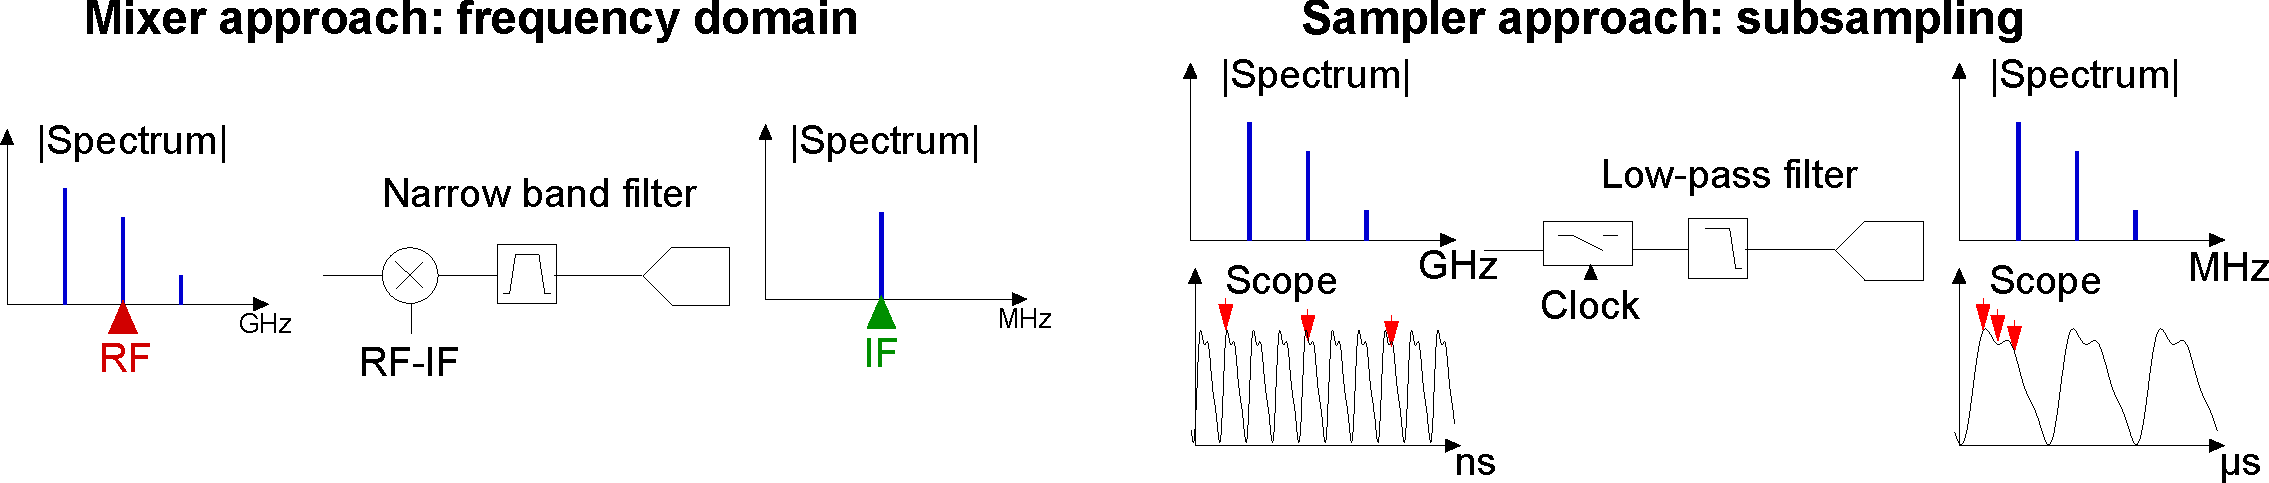
\includegraphics[width=1\linewidth]{RECEIVER.pdf}
\end{center}
}


%----------------------------------------------------------------------------------------
%	MEASUREMENT SETUP
%----------------------------------------------------------------------------------------
\headerbox{Measurement Setup for Envelope Tracking Application}{name=application,span=2,column=1,below=receiver}{ 
The setup includes \textbf{two LSNAs simultaneously}. One is dedicated to RF (sampler based downconversion), the other one samples directly the LF stimulus. The purpose is to investigate \textbf{low-frequencies $S_{22}$} of the DUT under RF large signal conditions.
\begin{center}
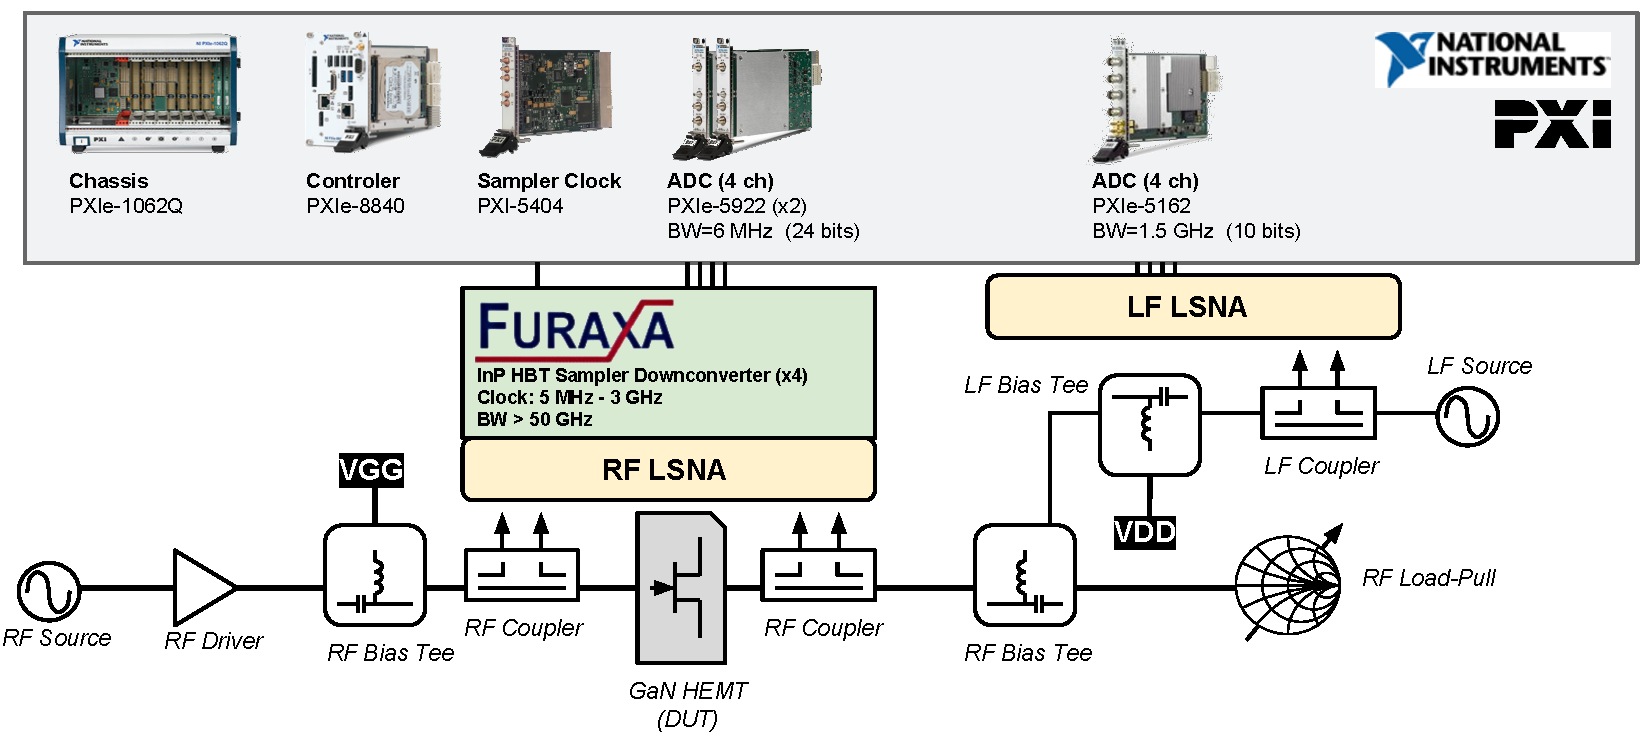
\includegraphics[width=\linewidth]{BENCH.pdf}
\small \textit{Low-frequency measurement of drain supply envelope-bandwidth impedance for supply-modulated PAs}
\end{center}
}


%----------------------------------------------------------------------------------------
%	CONCLUSION
%----------------------------------------------------------------------------------------
\headerbox{Conclusion}{name=conclusion,column=1,below=application,span=2}{
This new project will enable a new RF measurement capability by enabling an instrument that currently does not exist on the market. Some additional benefits include:
\vspace{-0.2cm}
\begin{itemize} 
\item frequency range extension of NI RF instrument products currently available;
\vspace{-0.2cm}
\item sampler architecture offers a unique multi-scale time analysis possibility (e.g. signal and carrier domains);
\vspace{-0.2cm}
\item can be implemented with various ADCs and downconverters (e.g. THAs);
\vspace{-0.2cm}
\item 100\% LabVIEW environment;
\vspace{-0.2cm}
\item goal is to offer open-source LabVIEW software for user measurement flexibility.
\end{itemize}
}


%----------------------------------------------------------------------------------------
%	REFERENCES
%----------------------------------------------------------------------------------------

%\headerbox{References}{name=references,column=2,below=application}{

%\smaller % Reduce the font size in this block
%\renewcommand{\section}[2]{\vskip 0.05em} % Get rid of the default "References" section title
%\nocite{*} % Insert publications even if they are not cited in the poster

%\bibliographystyle{unsrt}
%\bibliographystyle{IEEEtran}
%\bibliography{biblio} % Use biblio.bib as the bibliography file
%}


%----------------------------------------------------------------------------------------
%	ACKNOWLEDGEMENTS
%----------------------------------------------------------------------------------------

\headerbox{Acknowledgements}{name=acknowledgements,column=0,below=conclusion, above=bottom,span=3}{
\smaller 
This work is funded by National Instruments (Dr. Truchard) through a charitable donation. We would like to acknowledge DARPA (Dr. Greene) and ONR (Dr. Maki) for funding the initial part of this work under grant N00014-11-1-0931. \hfill \tiny \textit{Poster downloaded from} \textbf{www.microwave.fr}
} 


\end{poster}

\end{document}